\documentclass[12pt,letterpaper]{article}
\usepackage{amsmath} % just math
\usepackage{amssymb} % allow blackboard bold (aka N,R,Q sets)
\usepackage{ulem}
\usepackage{graphicx}
\usepackage{float}
\linespread{1.6}  % double spaces lines
\usepackage[left=1in,top=1in,right=1in,bottom=1in,nohead]{geometry}
\usepackage{caption}
\usepackage{subcaption}
\usepackage{floatrow}
\usepackage{blindtext}
\usepackage[table]{xcolor}

\begin{document}
\setcounter{subsection}{2} 
\begin{flushright}
\end{flushright}
\begin{flushleft}
\textbf{Eric Zounes} \\
\today \\ 
CS434: Assignment 3
\end{flushleft}

\begin{enumerate} 
	\item[1.] Association Rules. Given the following database of trasactions: \\
	\begin{center}
	\begin{tabular}{| l | c |}   
		\hline
		Transaction ID & Items \\ \hline
		1 & A,B  \\ \hline
		2 & A, B, C, D  \\ \hline
		3 & A, D, \\ \hline
		4 & C, D \\ \hline 
	\end{tabular} 
	\end{center} 
	\begin{enumerate} 
		\item[a.] Find all frequent itemsets with minimum support count $= 2$. Pease provide clear intermediate steps, indicating $C_{1},L_{1},C_{2},L_{2}, \ldots$ until the algorithm terminates. Be sure to include (and clearly indicate) the results of the self-join, and pruning step in generating candidate sets. \\
	
		\begin{tabular}{| l | c |}   
		\hline
		Item & $\sigma$ \\ \hline
	   \cellcolor{green}$A B$ & 2  \\ \hline
		$A C$ & 1  \\ \hline
		\cellcolor{green}$A D$ & 2 \\ \hline
		$B C$ & 1 \\ \hline 
		$B D$ & 1 \\ \hline 
		\cellcolor{green}$C D$ & 2 \\ \hline 
		\end{tabular} 	
		
		\item[b.] Find all association rules with miminum support count $= 2$ and min\_conf = $75$.  \\
		\begin{tabular}{| l | c |}   
		\hline
		Item & Conf. \\ \hline
		$A \rightarrow B$ & $\frac{2}{3}$  \\ \hline
		\cellcolor{green}$B \rightarrow A$ & 1  \\ \hline
		$A \rightarrow D$ & $\frac{2}{3}$ \\ \hline
		$D \rightarrow A$ & $\frac{2}{3}$ \\ \hline 
		\cellcolor{green}$C \rightarrow D$ & 1 \\ \hline 
		$D \rightarrow C$ & $\frac{2}{3}$ \\ \hline 
		\end{tabular} 	
				
	\end{enumerate} 
	\item[2.] Please consider the data provided on the class website, which is a 2 dimensional data that comes from a Gaussian distributino with a full covariance matrix. Apply PCA to this data. In particular, you need to first estimate the covariance matrix of this data, and the two PCA projection vectors (i.e., the eigen vectors of the covariance matrix). \\
	\begin{enumerate} 
		\item[a.] Report the covariance matrix that you estimated from the data. \\
				\begin{verbatim} 
					MATLAB code:
						M = csvread('pcs.csv')
						V = cov(M)
						  = 0.9301    0.8121
							0.8121    2.0456
				\end{verbatim} 
		\item[b.] Report the projection vectors for PC1 and PC2. \\
				\begin{verbatim} 	

				 [x1, x2] = eig(V)
					  x1 =
					     = -0.8849    0.4657
						0.4657    0.8849
					  x2 =
					        0.5027         0
					        0    	  2.4730
				\end{verbatim} 
		\item[c.] Please plot the data in two difference figures, one in the original 2-d coordinate system, and one in the PCA space(2-d). \\
	\pagebreak
	\end{enumerate}
	\begin{figure} 
	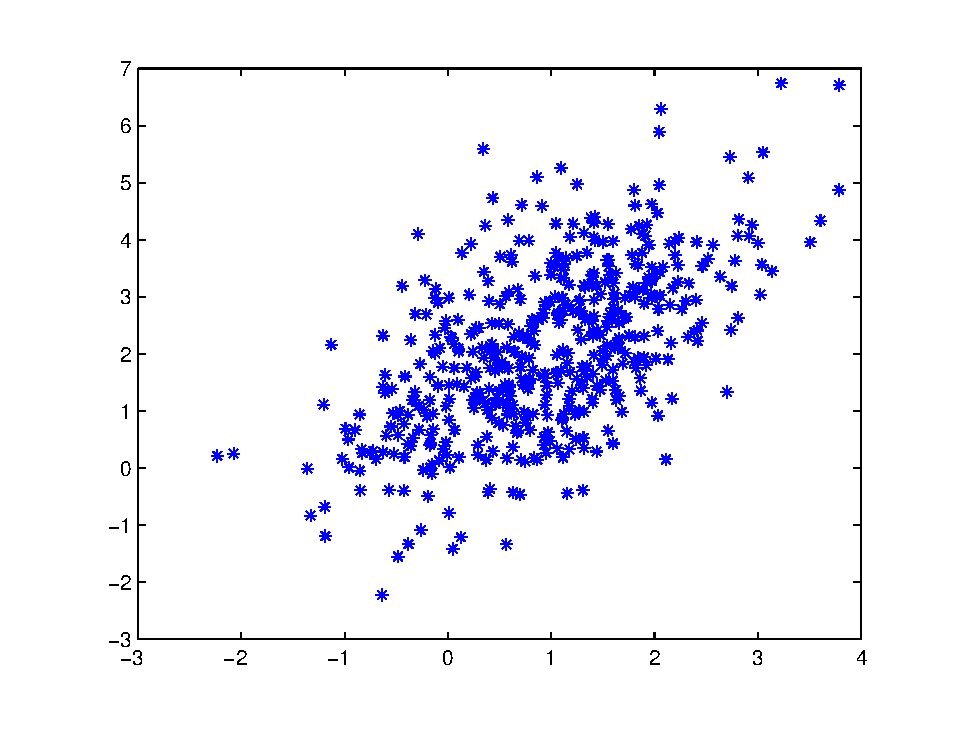
\includegraphics[width=6in]{original_2d.eps} 
	\caption{A plot of the data on the original 2d space.} 
	\end{figure}
	When we find the PCA vectors, we can change the axis of the data plot. \\
	\begin{figure} 
	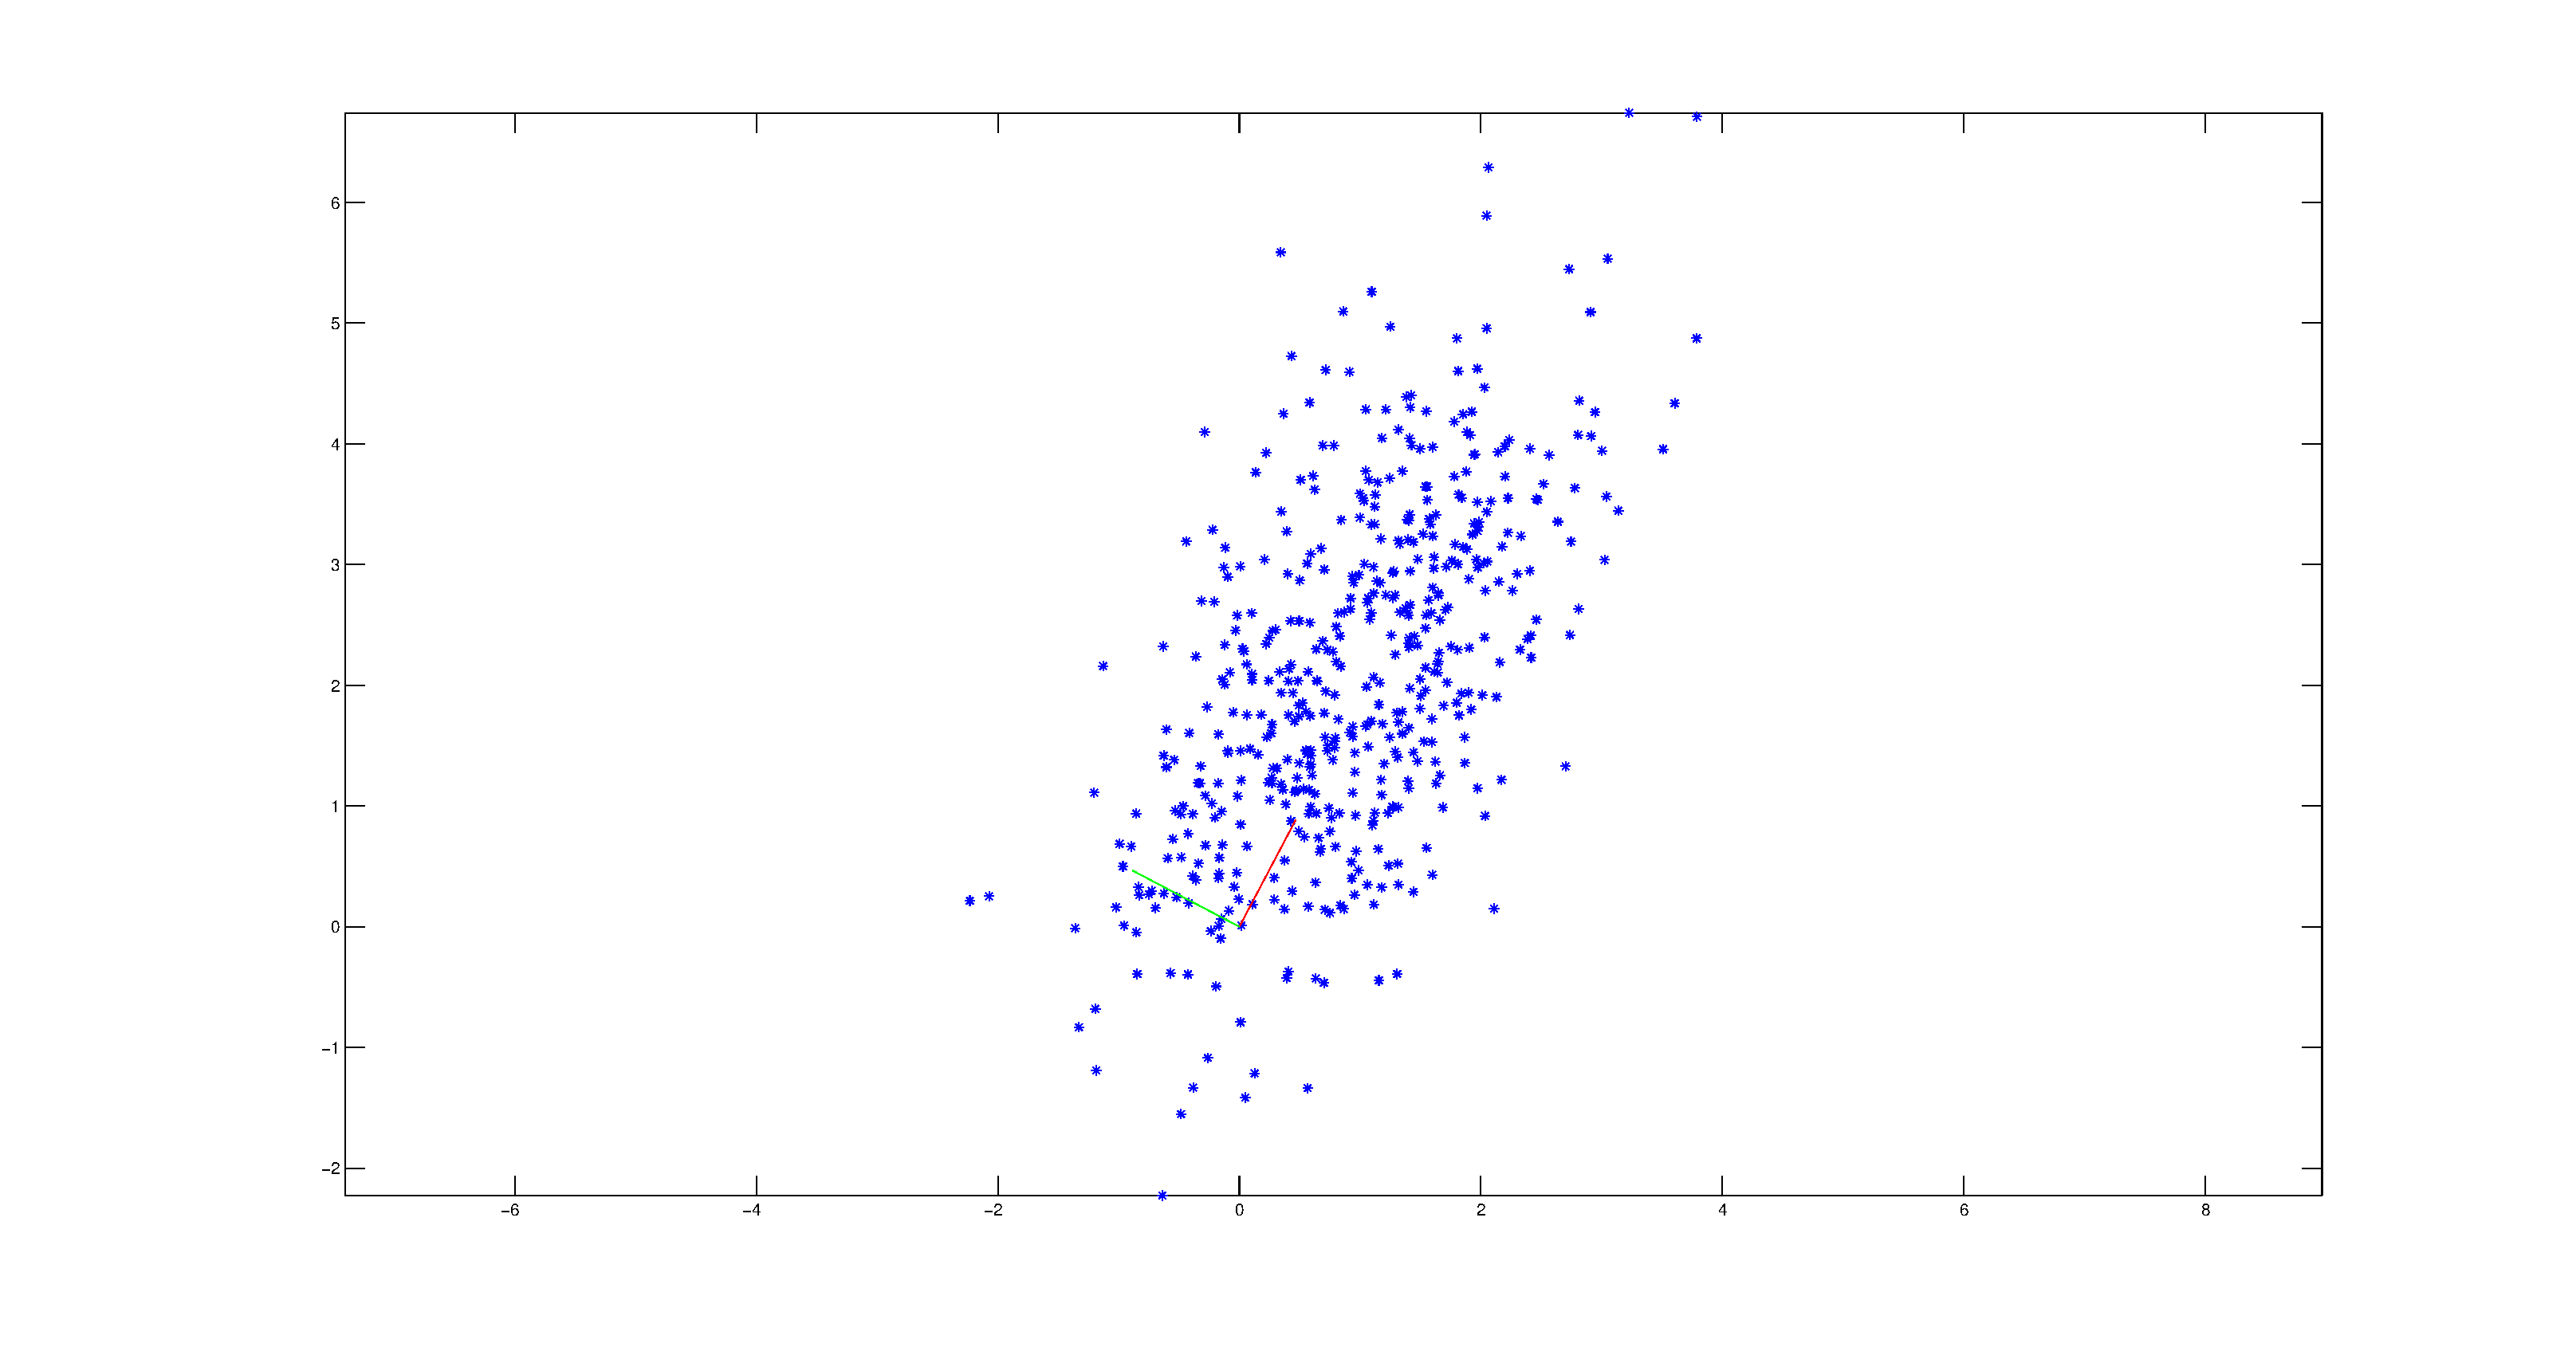
\includegraphics[width=6in]{pca_space.eps} 
	\caption{A plot of the data in PCA space.} 
	\end{figure}
	\end{enumerate}
	\pagebreak
	\item[3.] Given a dataset, PCA seeks to find a small number of dimensions that preserve as much variance in data as possible. Now consider a supervised learning task, can you come up with a situation where applying PCA to the data can significantly worsen the classification performance? In other words, is it possible to have data that is original separable but made non-separable by PCA projection (to lower dimension)? Please provide a visual example \\
\pagebreak	
	\item[4.] Boosting. Consider a data set $D = {x_{1},x_{2},\ldots,x_{10}}$. We apply Adaboost with Decision Stump. Let $w_{1}, \ldots, w_{10}$ be the weights of the ten training examples respectively. \\
	\begin{enumerate}
		\item[a.] In the first iteration $, x_{1}, x_{2},$and$ x_{3}$ are misclassified. Please rank the updated weights $w_{1}, \ldots, w_{10}$ be the weights of the ten training examples respectively. \\
		$\epsilon_{1} = \frac{3}{10}$ \\
		$\alpha_{1} = \frac{1}{2} ln (\frac{1 - .3}{.3})$ \\
		$\alpha_{1} = .4236$ \\
		
		Updated rank: \\ 
			
		$D_{t+1}(i) = D_{t}(i) \times \begin{cases} e^{\alpha_{t}}, h_{t}(x_{t}) \neq y_{t} \\ e^{\alpha_{t}}, h_{t}(x_{t}) = y_{t} \end{cases}$ \\[10mm]
		

		$w_{4}, w_{5}, w_{6}, w_{7}, w_{8}, w_{9}, w_{10}, w_{1}, w_{2}, w_{3}$ \\
			
		\item[b.] In the second iteration, $x_{3}$ and $x_{4}$ are misclassified. Please provide the rank of the updated weights $w_{1}, \ldots, w_{10}$ in increasing order. Explain your ordering. \\
		
		$\epsilon_{t} = x_{4} + x_{3} $ \\
		$\epsilon_{2} = \frac{1}{10} + .1527 $ \\
		$\epsilon_{2} = .252$ 
		$\alpha_{2} = \frac{1}{2} ln (\frac{1 - .252}{.252})$ \\
		$\alpha_{2} = .544$ \\
		
		Updated rank: \\
		
			$D_{t+1}(i) = D_{t}(i) \times \begin{cases} e^{\alpha_{t}}, h_{t}(x_{t}) \neq y_{t} \\ e^{\alpha_{t}}, h_{t}(x_{t}) = y_{t} \end{cases}$ \\[10mm]
		
	$w_{4} = .1723, w_{3} = .2631$ 	\\
	
	$w_{5}, w_{6}, w_{7}, w_{8}, w_{9}, w_{10}, w_{1}, w_{2}, w_{4}, w_{3}$ \\

	\end{enumerate}
\end{enumerate}
\end{document} 
